\section{Détermination de la courbe en S}
%_______________________________________
\subsection*{Présentation du problème}
\begin{frame}
\frametitle{Mise en équation}

   \begin{itemize}
      \item Équation thermique
      \begin{equation}
         Cv\frac{\partial T}{\partial t} = Q^+ + Q^- +Q^{adv}
      \end{equation}
      
   \item Équilibre thermique local
   \begin{equation}
      Q^+ = Q^- 
   \end{equation}
   
      \begin{itemize}
         \item état stationnaire
         \\
         \item dépend de la position
         \item courbes en S pour 256 valeurs du rayon
      \end{itemize}
\end{itemize}
\end{frame}
%_______________________________________

%_______________________________________
\subsection*{Résolution des équations}
\begin{frame}
\frametitle{Résolution des équations}

   \begin{itemize}
      \item Ordre des équations
      \item Détermination de la température
      \item Méthodes de résolution
         \begin{itemize} 
            \item Dichotomie
            \item Amélioration de la dichotomie
            \item Méthode de Brent
            \item Comparaison des différentes méthodes
         \end{itemize}
      \item Épaisseur optique
   \end{itemize}
\end{frame}
%_______________________________________

%_______________________________________

%_______________________________________
\begin{frame}
\frametitle{Ordre des équations}
      
   \begin{figure}[htb!]
      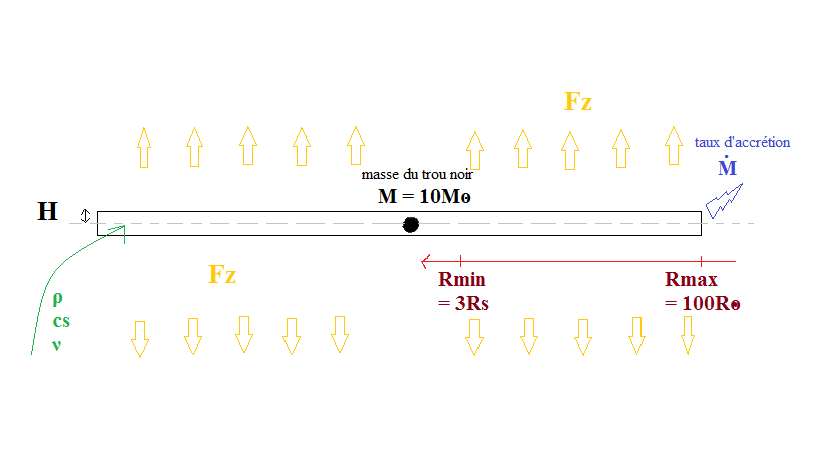
\includegraphics[width=9cm]{figures/bob_ross.png}
      \caption{Schéma très simplifié du disque d'accrétion autour d'un trou noir.}
   \end{figure}      
      \end{frame}

\begin{frame}
\frametitle{Ordre des équations}
         \begin{itemize}
      \item Demi-hauteur H du disque

      Solution d'une équation quadratique trouvée à partir de la pression :
      \begin{equation}
         P = P_\mathrm{gaz} + P_\mathrm{rad}
      \end{equation}
      \item Densité volumique $\rho$
      \item Vitesse du son $c_s$ 
      \item Viscosité $\nu$ 
      \item Flux radiatif $F_z$
      \\
      2 approximations en fonction de la profondeur optique $\tau_{eff}$
   \end{itemize}
\end{frame}
%_______________________________________


%_______________________________________

\begin{frame}
\frametitle{Détermination de l'intervalle de Température} 
Luminosité d'Eddington
   \begin{equation}
      L_\mathrm{Edd} = \frac{4\pi GMm_pc}{\sigma_e}
   \end{equation}

Taux d’accrétion critique 
   \begin{equation}
      \dot{M}_\mathrm{crit} = \frac{12}{c^2}L_\mathrm{Edd} 
   \end{equation}

Température caractéristique $T_0$
   \begin{equation}
      T_0 \approx 2,50.10^7\left(\frac{\dot{M}_0}{\dot{L}_\mathrm{crit}}\right)^{\frac{1}{4}}\left(\frac{M}{M_\odot}\right)^{-\frac{1}{4}} \mathrm{K}
   \end{equation}


\end{frame}
%_______________________________________


%_______________________________________

%\begin{frame}
%\frametitle{Détermination de l'intervalle de Température} 

 %  Finalement : 
%\begin{eqnarray}


 %  T_0 =1.40\ 10^6 \mathrm{K} 
   
 %  T_\textrm{min} = 2.9\ 10^5 \mathrm{K}
    
 %  T_\textrm{max} = 6.2\ 10^6 \mathrm{K} 
%\end{eqnarray}

%\end{frame}
%_______________________________________


%_______________________________________

\begin{frame}
\frametitle{Dichotomie}

   \begin{itemize}
      \item Racine $f(\Sigma) = Q^+ - Q^- = 0$ comprise dans un intervalle $[\Sigma_{min}$ ; $\Sigma_{max}]$
      \\
      \begin{figure}[htb!]
         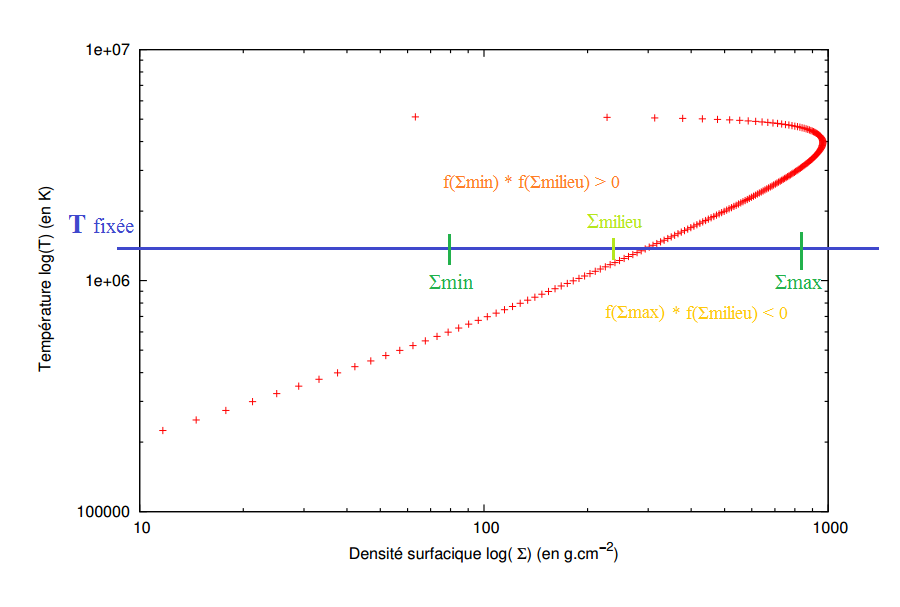
\includegraphics[width=8cm]{figures/dicho_1.png}
      \end{figure}
   \end{itemize}
\end{frame}
%_______________________________________

%_______________________________________

\begin{frame}
\frametitle{Dichotomie}

   \begin{itemize}
      \item Racine $f(\Sigma) = Q^+ - Q^- = 0$ 
      
      comprise dans un intervalle $[\Sigma_{min}$ ; $\Sigma_{max}]$
      \\
      \begin{figure}[htb!]
         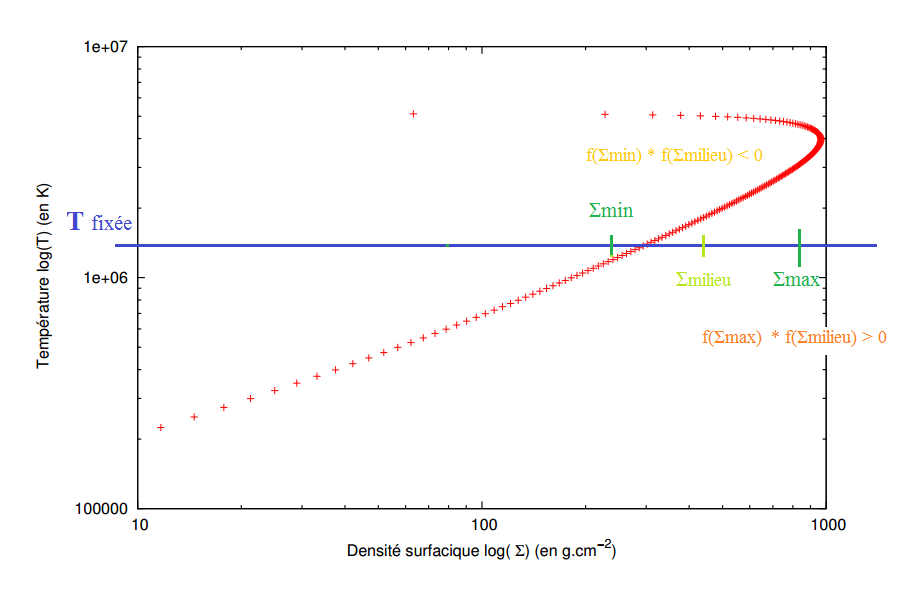
\includegraphics[width=8cm]{figures/dicho_2.png}
      \end{figure}
   \end{itemize}
\end{frame}
%_______________________________________


%_______________________________________

\begin{frame}
\frametitle{Amélioration de la dichotomie}
\framesubtitle{Méthode de Newton}
%\setbeamertemplate{itemize item}[square]

   \begin{itemize}
      \item Présentation
      \\
      \begin{equation}
         x_{k+1} = x_k - \frac{f(x_k)}{f'(x_k)}
      \end{equation}

      \begin{figure}[htb!]
         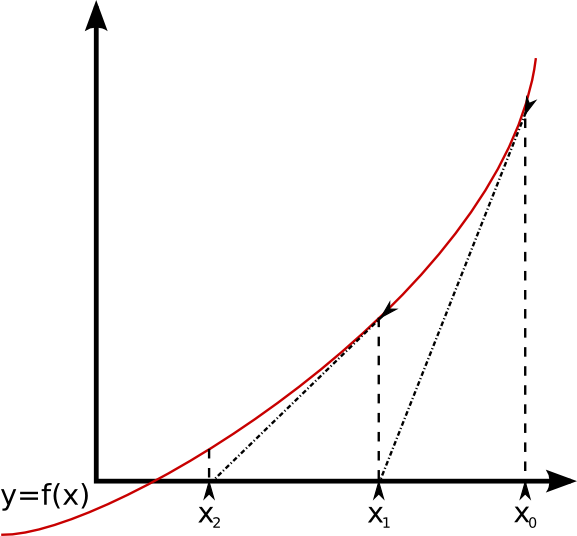
\includegraphics[width=3cm]{figures/Newton_method.png}
         \caption{Illustration de la méthode de Newton. Crédit: Wikimedia Commons}
      \end{figure}

   \end{itemize}
\end{frame}
%_______________________________________

%_______________________________________

\begin{frame}
\frametitle{Amélioration de la dichotomie}
\framesubtitle{Méthode de Newton}
%\setbeamertemplate{itemize item}[square]

   \begin{itemize}
      \item Avantages :
         \begin{itemize}
            \item Convergence quadratique
         \end{itemize}
      \item Inconvénients :
      \begin{itemize}
         \item Nécessite le calcul littéral de la dérivée.
         \item La fonction doit être obligatoirement de classe $C^1$.
         \item S'il existe plusieurs racines, ne converge pas forcément vers la plus proche du point de départ.
      \end{itemize}
   \end{itemize}
\end{frame}
%_______________________________________




%_______________________________________
\begin{frame}
\frametitle{Méthode de la sécante}


Approximation de la méthode de Newton par
    \begin{equation}    
f'(x_n) \approx  \frac{f(x_{n}) - f(x_{n-1})}{x_{n}-x_{n-1}}        
    \end{equation}  
     
 
Ce qui donne
     \begin{equation}
        x_{n+1} = x_n - \frac{x_n - x_{n-1}}{f(x_n) - f(x_{n-1})}
     \end{equation}

\end{frame}
%_______________________________________





%_______________________________________
\begin{frame}
\frametitle{Méthode de Brent}

Combinaison des méthodes de la dichotomie, de la sécante et l'interpolation quadratique inverse pour en utiliser tous leurs avantages.

   \begin{itemize}
      \item Méthode quadratique inverse
    \begin{equation}\begin{aligned}
         x_{n+1} &= \frac{f(x_{n-1})f(x_n)}{(f(x_{n-2})-f(x_{n-1}))(f(x_{n-2})-f(x_{n}))}x_{n-2} \\
         &+  \frac{f(x_{n-2})f(x_n)}{(f(x_{n-1})-f(x_{n-2}))(f(x_{n-1})-f(x_{n}))}x_{n-1} \\
         &+ \frac{f(x_{n-2})f(x_{n-1})}{(f(x_{n})-f(x_{n-2}))(f(x_{n})-f(x_{n-1}))}x_{n} \\
    \end{aligned}
    \end{equation}  
     

   \end{itemize}
\end{frame}
%_______________________________________


%_______________________________________

\begin{frame}
\frametitle{Méthode de Brent}

   \begin{itemize}
      \item Si dénominateur $\ne$ 0 méthode quadratique inverse.
      \item Sinon méthode de la sécante sauf si l'on est trop éloigné de la solution.
      \item Dans ce cas, on utilise la méthode de la dichotomie.
   \end{itemize}
\end{frame}
%_______________________________________


%_______________________________________

\begin{frame}
\frametitle{Comparaison des différentes méthodes}

   \begin{figure}[htb!]
      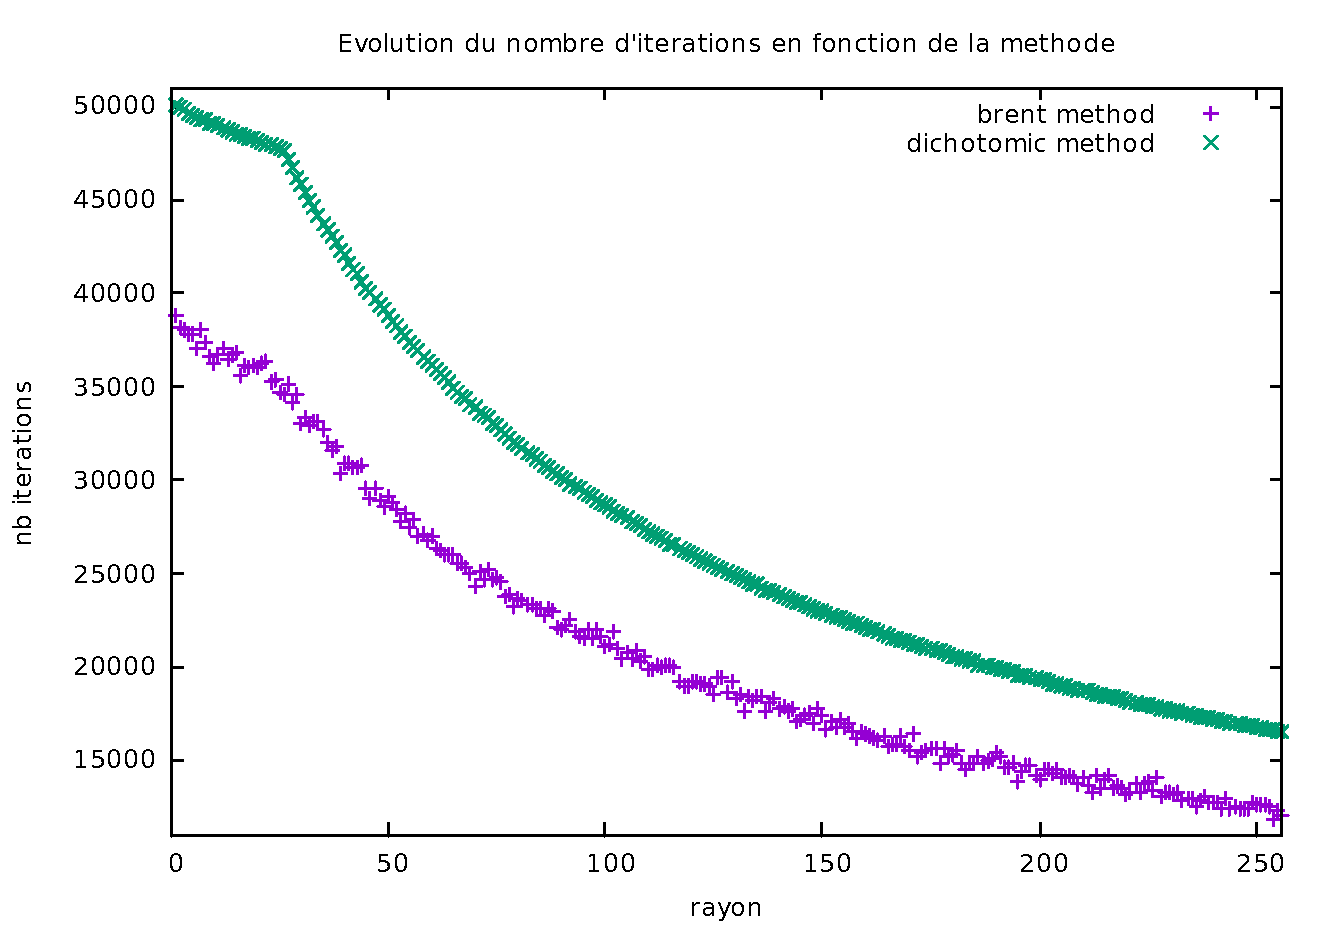
\includegraphics[width=9cm]{figures/brent_method3.pdf}
   \end{figure}
\end{frame}
%_______________________________________

%_______________________________________

\begin{frame}
\frametitle{Comparaison des différentes méthodes}

   \begin{tabular}{|c|c|c|}
     \hline
        Méthode & + & - \\
     \hline
     \\
     Dichotomie & simple & beaucoup d'itérations  
     \\  
     \hline
     \\
     Newton & plus rapide  & fonction dérivable 
     \\ 
     \hline
     \\  
     Sécante & pas de dérivée & intervalle de départ 
     \\  
     \hline  
     \\  
     Brent & interpolation quadratique inverse & convergence rapide 
     \\  
     \hline
   \end{tabular}
\end{frame}
%_______________________________________


%_______________________________________

\subsection*{Détermination des points critiques}
\begin{frame}
\frametitle{Zones de stabilité}

   \begin{figure}[htb!]
      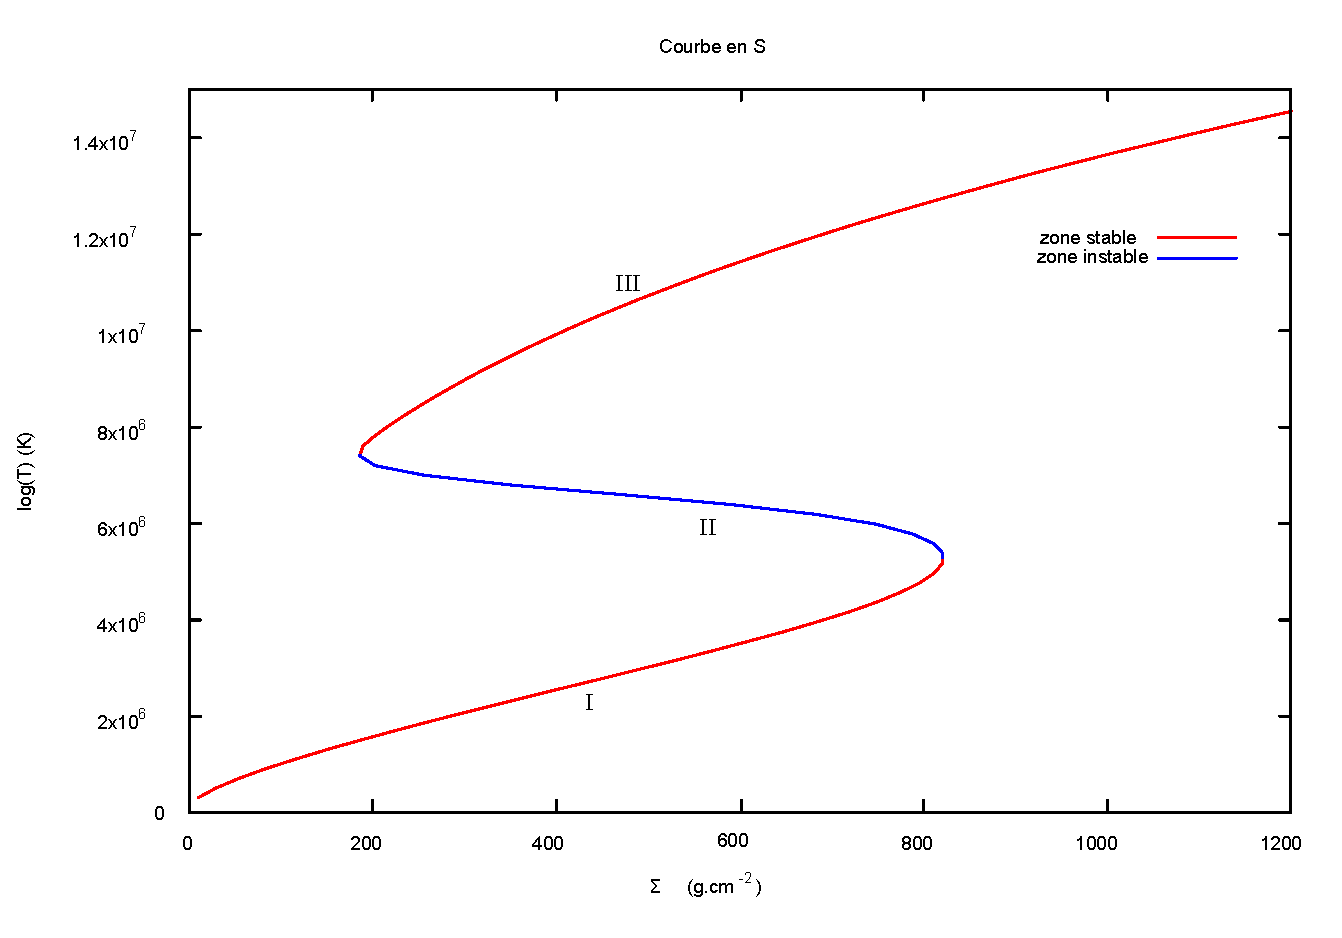
\includegraphics[width=9cm]{figures/stable.pdf}
      %LOG!!!
      \caption{Zones de stabilités de la courbe en S.}
    \end{figure}
\end{frame}
%_______________________________________

\begin{frame}		
\frametitle{Points critiques}		
		
   \begin{figure}[htb!]		
      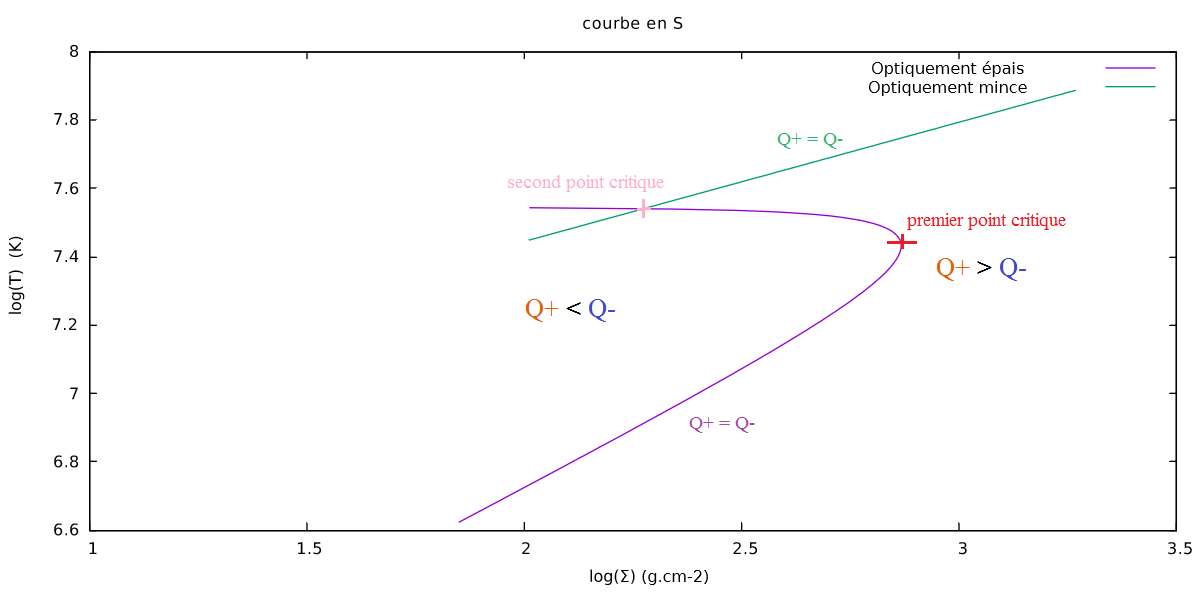
\includegraphics[width=8cm]{figures/points_critiques.png}		
      \caption{Localisation des points critiques sur la courbe en S.}		
    \end{figure}		
\end{frame}		


%_______________________________________

\subsection*{Épaisseur optique}
\begin{frame}

   \begin{figure}[htb!]
      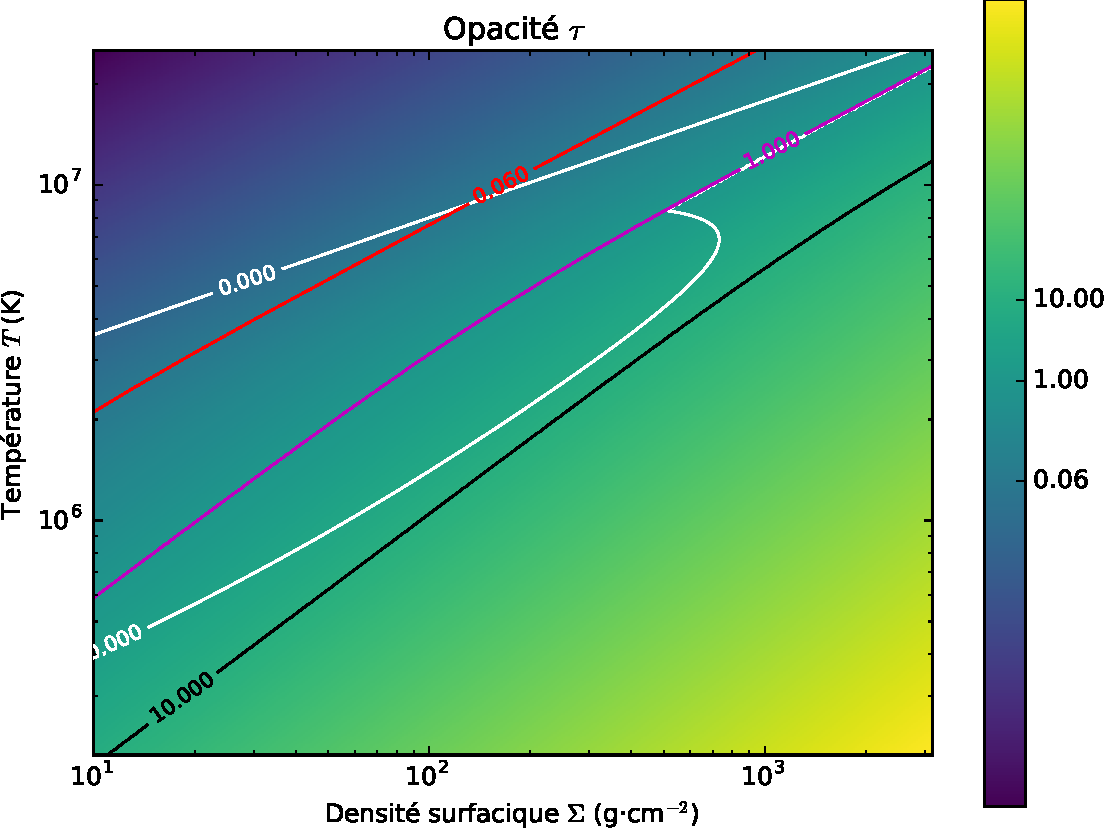
\includegraphics[width=8cm]{figures/tau_map.pdf}
      %\caption{ }
   \end{figure}
\end{frame}
%_______________________________________

%_______________________________________
\subsection*{Différence des termes Q+ et Q-}
\begin{frame}

   \begin{figure}[htb!]
      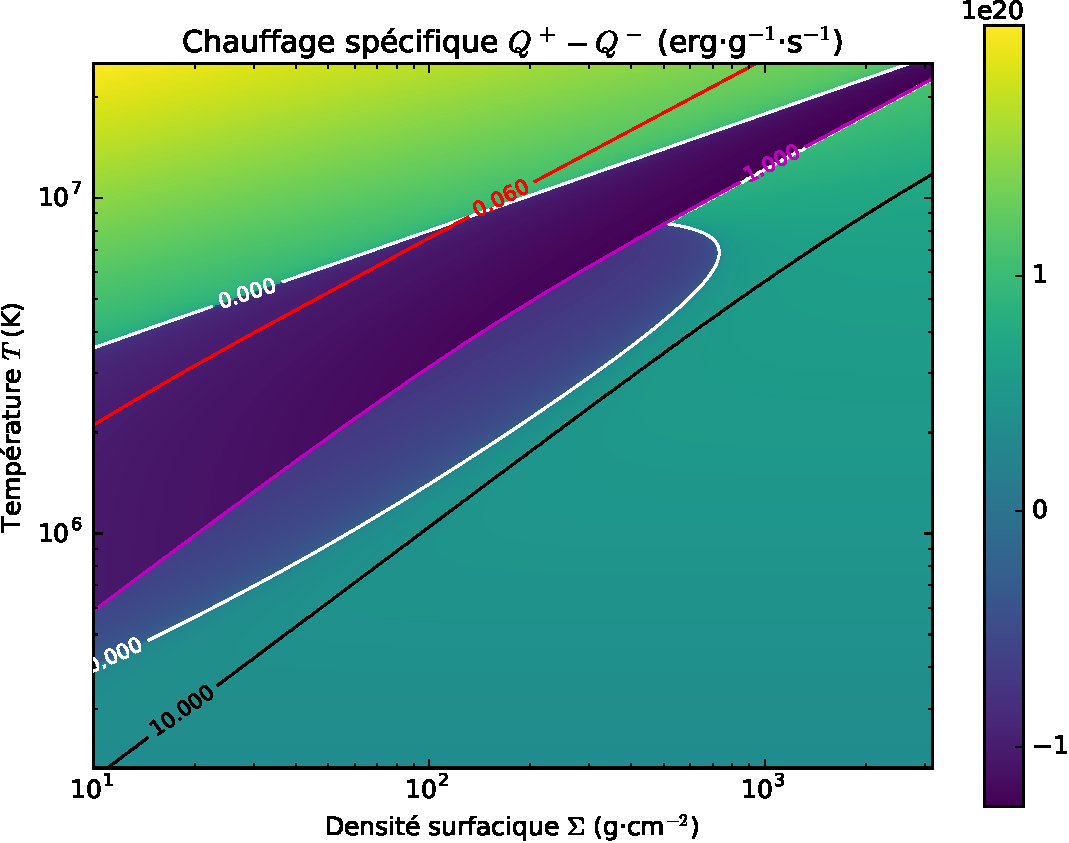
\includegraphics[width=8cm]{figures/Qmap.pdf}
     %\caption{ }
   \end{figure}
\end{frame}
%_______________________________________

%_______________________________________

\subsection*{Discussion et conclusion}
\begin{frame}

   \begin{itemize}
      \item Non unicité des racines de $f(\Sigma) = 0$
      \\
         \begin{itemize}
            \item Interpolation du $\tau_{eff} \approx 1$ critique
            \item Existance de plusieurs branches minces ? 
         \end{itemize}  
      \item $\tau_{eff} \simeq 0.06 et \neq 1$ 
      \\
Simulation en accord avec la valeur théorique
   \end{itemize}
\end{frame}
%_______________________________________

%_______________________________________

\begin{frame}

   \begin{figure}[htb!]
      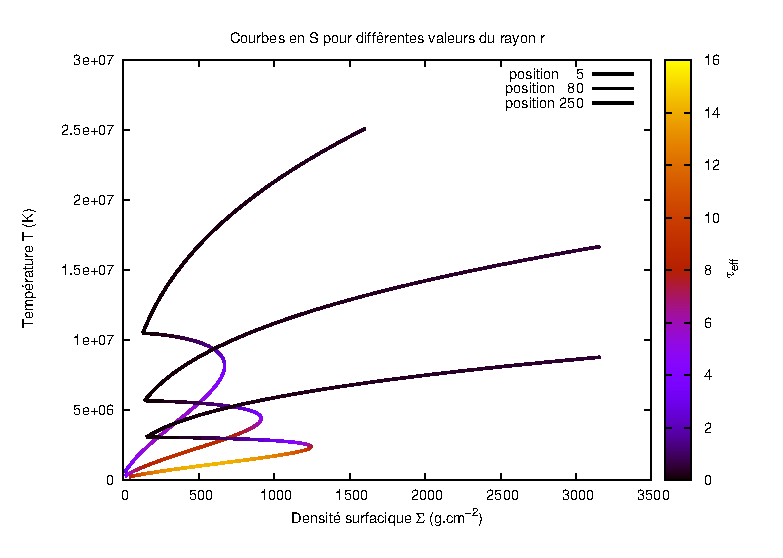
\includegraphics[width=9cm]{figures/S_curves_tau.eps}
      %\caption{ }
   \end{figure}
\end{frame}
%_______________________________________